\chapter{Machine Learning Pipelines}
\label{ch:ml-pipeline}
Recall the pipeline diagram from the first chapter.

\begin{figure}[h]
  \centering
  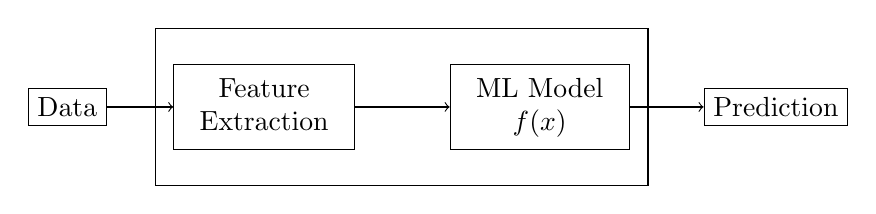
\begin{tikzpicture}
    \node[draw, rectangle] (data) at (0, 0) {Data};
    \node[draw, rectangle] (features) at (2.5, 0) {\begin{tabular}{c}Feature\\Extraction\end{tabular}};
    \node[draw, rectangle, minimum height=2cm, minimum width=6.25cm] () at (4.25, 0) {};
    \node[draw, rectangle] (model) at (6, 0) {\begin{tabular}{c}ML Model\\$f(x)$\end{tabular}};
    \node[draw, rectangle] (prediction) at (9, 0) {Prediction};
    \draw[->] (data) -- (features);
    \draw[->] (features) -- (model);
    \draw[->] (model) -- (prediction);
  \end{tikzpicture}
  \caption{Machine Learning Pipeline}
  \label{fig:ml-pipeline}
\end{figure}
Up until now we always assumed to have a vector representation $\vec{x}\in\mathbb{R}^d$ of our data.
Starting from now, our data might be in any other format, like text or images.

To build a system that gets a certain format of input, transform this input into $d$ dimensional vectors and feeds them into our model.
We will now look at how to program such an ML-Pipeline
\section{Motivation}
In the previous chapters we looked into different feature extraction techniques.
We also looked in previous chapters into different ML models and how to train them.
Now, we will look into how to combine these two concepts into a single pipeline.

One way how to implement this is to manually write code that executes all steps of the pipeline sequentially.
But this would be quite static and not very flexible. We would need to rewrite the code for every new data set or whenever
we want to change a part of the pipeline.

A better way to implement this is to use a so called \textit{Pipeline} object. This object is a wrapper around all steps of the pipeline.
The most popular API-Interface~\cite{sklearn_api} for this is implemented by the guys from scikit-learn~\cite{scikit-learn}.

We will look into the implementation of such a pipeline in the following because it will allow to combine
own implementations with implementations inside scikit-learn. This is especially useful because scikit-learn
delivers plenty of tools, feature extraction algorithms and model architectures.

I personally work a lot with scikit-learn and I highly recommend it to anyone who wants to get started with ML as well assigned
encourage everyone to contribute to the project.

\section{Estimators}
The basic concept of the scikit-learn API are so called \textit{Estimators}, which define a overall interface for all sorts of algorithms, like classifiers or feature extractors.
Each estimator implements a \lstinline{fit} method, which takes a data set as input and learns from it. A \lstinline{transform} method that applies the estimator to data which can yield classification predictions or transformed data.
And optionally a \lstinline{set_params} and a \lstinline{get_params}-method to set and get configuration of the estimator.

\textbf{Example}\\
Imagine we want to detect \textit{spam} in emails. Doing so we would end up with a pipeline similar to the one in figure~\ref{fig:ml-pipeline-spam}.

\begin{figure}[h]
  \centering
  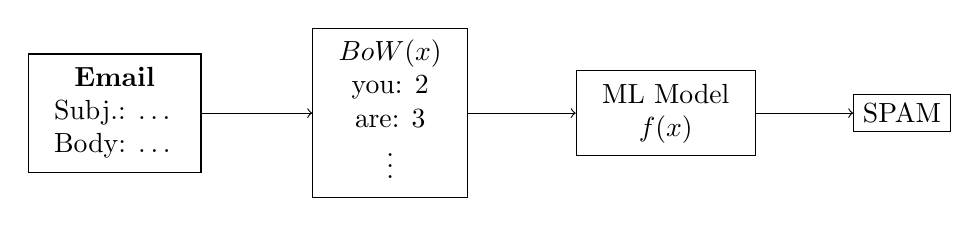
\begin{tikzpicture}
    \node[draw, rectangle] (data) at (-1, 0) {\begin{tabular}{c}\textbf{Email}\\Subj.: \dots\\Body: \dots\end{tabular}};
    \node[draw, rectangle] (features) at (2.5, 0) {\begin{tabular}{c}$\text{BoW}(x)$\\you: 2\\are: 3\\\vdots\end{tabular}};
    \node[draw, rectangle] (model) at (6, 0) {\begin{tabular}{c}ML Model\\$f(x)$\end{tabular}};
    \node[draw, rectangle] (prediction) at (9, 0) {SPAM};
    \draw[->] (data) -- (features);
    \draw[->] (features) -- (model);
    \draw[->] (model) -- (prediction);
  \end{tikzpicture}
  \caption{Machine Learning Pipeline for Spam Detection}
  \label{fig:ml-pipeline-spam}
\end{figure}

\section{Pipelines}
To build a full \textit{Pipeline} object, we can chain Estimators to run sequentially. This allows combining Feature Extractors and Classifiers into a full Pipeline object.
Once chained, the Pipeline works just like an Estimator itself. It has a \lstinline{fit} and a \lstinline{transform} method. The \lstinline{fit} method will call the \lstinline{fit} method of each estimator in the pipeline sequentially.
A second big advantage of such Pipeline object is that all parameters of it can be optimized jointly. This means that we can optimize the parameters of the feature extractor and the classifier at the same time.
This Pipeline approach is great and allows us to quickly train and run full ML systems/architectures.\\
15-20 years ago, people needed to code all of this from scratch, in C.
So nowadays we must appreciate this great work and use it to our advantage.\\
Recently we see a new spring of manual implementations of ML algorithms, especially in C and C++.
With the publication of OpenAI's Whisper~\cite{radford2022whisper} or the leak of the weights of Meta's first generation of LLaMa~\cite{llama} and the release of the second generation of LLaMa~\cite{llama2} we see a lot of people trying to implement and hack ML models from scratch, such as
\begin{itemize}
  \item \href{https://github.com/karpathy/llama2.cpp}{llama2.cpp} by Andrej Karpathy
  \item \href{https://github.com/ggerganov/llama.cpp}{llama.cpp} by Georgi Gerganov
  \item \href{https://github.com/ggerganov/whisper.cpp}{whisper.cpp} by Georgi Gerganov
\end{itemize}

\framedtext{\color{red}{TODO:}}

